\chapter{\IfLanguageName{dutch}{Ontwikkeling en training van objectdetectiemodellen}{Datacollection and Labeling}}
\label{ch:objectdetectie}

\section{Doelstelling}
Deze fase was gericht op het ontwikkelen en trainen van geavanceerde objectdetectiemodellen om koeien en hun gedragingen nauwkeurig te identificeren binnen diverse agrarische omgevingen.

\section{Methoden}
\begin{itemize}
  \item \textbf{Voorbereiding van data:} De uit Labelbox geëxtraheerde data moest worden omgezet naar verschillende formats geschikt voor elk specifiek model. Voor YOLO-modellen was dit proces relatief eenvoudig vanwege het algemene formaat en de beschikbaarheid van vooraf gemaakte functies die de conversie automatiseren. Echter, voor Detectron's Faster R-CNN en SSD moest de data nauwgezetter worden aangepast om aan hun specifieke invoervereisten te voldoen, wat het proces complexer en tijdrovender maakte.
  \item \textbf{Modelselectie en training:}
  \begin{itemize}
    \item \textbf{YOLO (You Only Look Once):} YOLO-modellen \textcite{Jocher_Ultralytics_YOLO_2023} zijn gekozen vanwege hun efficiëntie in real-time objectdetectie, die vooral belangrijk is voor toepassingen binnen de agrarische sector. Deze modellen zijn getraind op de voorgetrainde COCO dataset, wat hen een brede basis geeft voor het herkennen van diverse objecten. De training van alle YOLO-modellen werd uitgevoerd over 1000 epochs met een early stopping patience van 200 epochs. De meeste modellen bereikten convergentie na ongeveer 300 epochs. De hyperparameters werden standaard gehouden zonder verdere tuning door de lange trainingstijden; bijvoorbeeld, de training van YOLOv9 duurde 25 uur. Alle modellen werden getraind op het ILVO AI workstation met een Nvidia A100 GPU van 25 GB, wat aanzienlijke rekenkracht bood. Onze experimenten toonden aan dat YOLO-modellen snel reageren, met verwerkingstijden die niet meer dan 30 ms per beeld vereisen, en dat ze robuuste prestaties leveren op onze gespecialiseerde agrarische dataset.
    \item \textbf{Detectron's Faster R-CNN:} Detectron-modellen, bekend om hun nauwkeurigheid door de integratie van een Region Proposal Network gevolgd door een Fast R-CNN detector, zijn eveneens getest. Deze modellen zijn ook getraind met een voorgetrainde configuratie van de COCO-dataset, die uitstekend is voor het ontwikkelen van een diepgaand inzicht in verschillende objecttypes. Echter, ondanks hun hoge nauwkeurigheid, met een accuracy van 96.8\%, was de reactietijd van 759 ms per beeld te langzaam voor real-time besluitvorming in de agrarische sector.   
    \item \textbf{SSD (Single Shot Detector):} De Single Shot Detector (SSD) benadering wordt vaak gezien als een fundament voor complexere modellen zoals YOLO. Deze methode, hoewel effectief voor objectdetectie, vereist aanzienlijke inspanning in termen van het ontwikkelen van specifieke algoritmes voor het berekenen van prestatie-metrieken, noodzakelijk voor de evaluatie en vergelijking van het model met andere modellen. Bij de implementatie van SSD ontdekte ik dat de gebruiksvriendelijkheid niet mee zit, voornamelijk vanwege de noodzaak om aangepaste algoritmes te schrijven voor het berekenen van de loss. Na 10 epochs bereikte mijn model een loss van slechts 0.37\%, wat de potentie aantoont. Echter, door de tijdrovende en complexe opzet heb ik besloten dit model niet verder te onderzoeken voor mijn projecten.
  \end{itemize}
  \item \textbf{Complexiteit bij vergelijken van modelarchitecturen:} Het vergelijken van verschillende modelarchitecturen zoals YOLO en Detectron's Faster R-CNN brengt significante uitdagingen met zich mee, voornamelijk door het verschil in de soorten outputmetrics. YOLO-modellen worden beoordeeld op basis van precision en MAP (Mean Average Precision) scores, terwijl Detectron-modellen primair focussen op accuracy. Dit verschil in evaluatiemethodiek maakt het moeilijk om een directe en eerlijke vergelijking te trekken tussen de prestaties van de modellen, wat de besluitvorming over het optimale model voor specifieke toepassingen moeilijker maakt.
  \item \textbf{Reden voor focus op YOLO:} Gezien de verschillen in de vereiste inspanningen voor dataconversie, de complexiteit van de training en implementatie, en de verschillende outputmetrics die moeilijk te vergelijken zijn, hebben we besloten ons te concentreren op YOLO-modellen. Deze keuze werd gedreven door hun gebruiksgemak en de mogelijkheid om snel aanpassingen en optimalisaties door te voeren, wat essentieel is voor de dynamische omgeving van agrarische toepassingen.
\end{itemize}
\section{Vergelijking van verschillende YOLO-modellen}
Deze sectie presenteert een systematische vergelijking van verschillende varianten van YOLO-modellen die tijdens dit onderzoek zijn getraind. Doel is om te bepalen welk model het meest geschikt is voor de nauwkeurige detectie van koeiengedrag binnen mijn dataset.
\subsection{Vergelijkingsresultaten}
\begin{itemize}
\item \textbf{Prestatieanalyse:} Voor elk model worden gedetailleerde statistieken verstrekt over de meetcriteria. Grafieken en tabellen kunnen worden gebruikt om de prestaties visueel te vergelijken.
\item \textbf{Algemene aanbeveling:} Uit de vergelijking blijkt dat YOLOv9 de hoogste nauwkeurigheid behaalt. Echter, vanwege de relatief lange verwerkingstijd per beeld is YOLOv9 mogelijk minder geschikt voor toepassingen die real-time responsiviteit vereisen.
\item \textbf{Aanbevolen model voor optimale prestaties:} Vooor een betere balans tussen nauwkeurigheid en verwerkingssnelheid wordt YOLOv8large aanbevolen. Dit model biedt een uitstekende nauwkeurigheid die vergelijkbaar is met YOLOv9c, maar met een aanzienlijk snellere verwerkingstijd, waardoor het geschikter is voor real-time objectdetectietoepassingen.
% \item 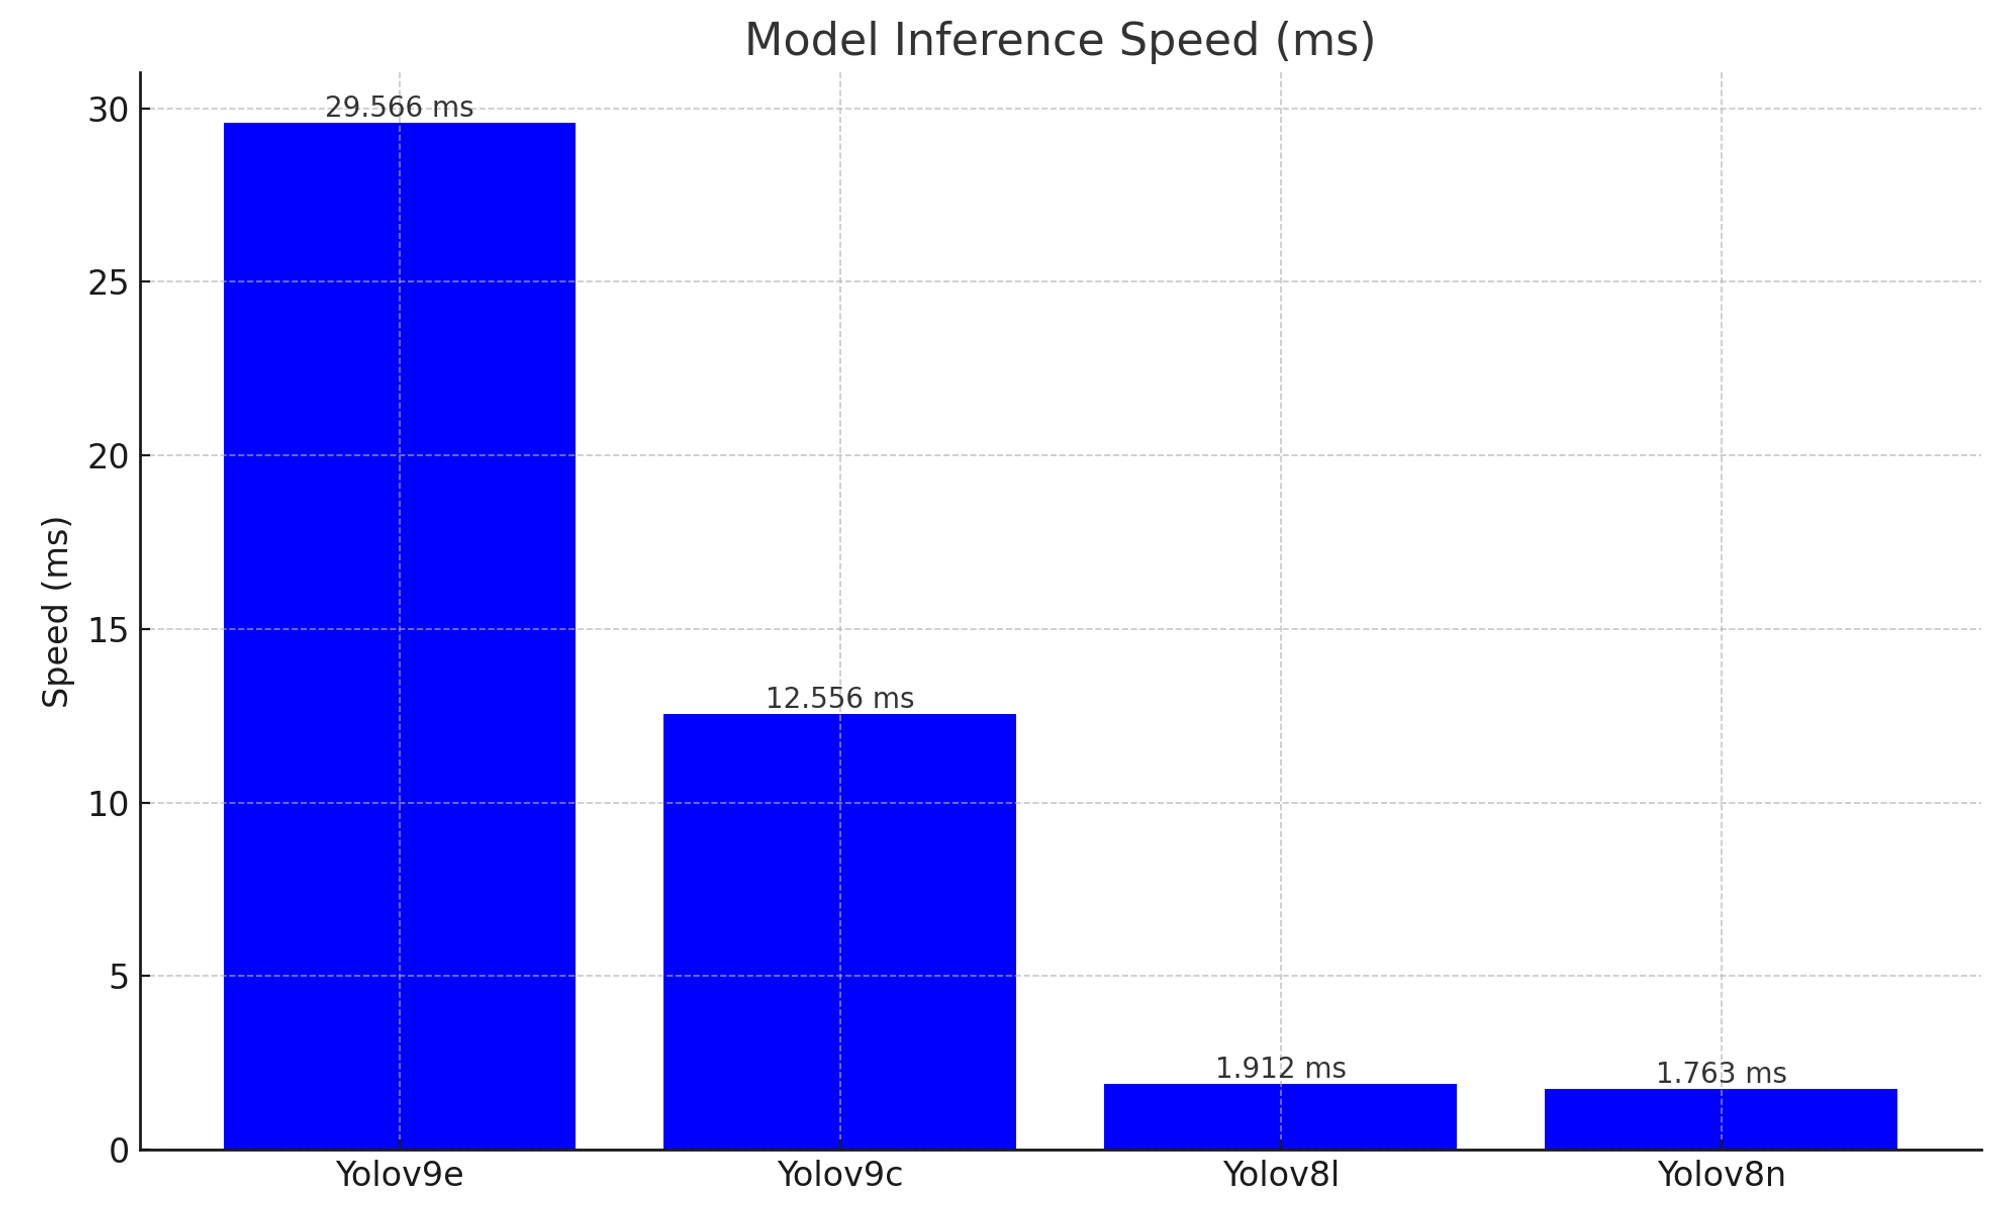
\includegraphics[width=\linewidth]{objectdetectie_yolo_metrics_speed.png}
% \item 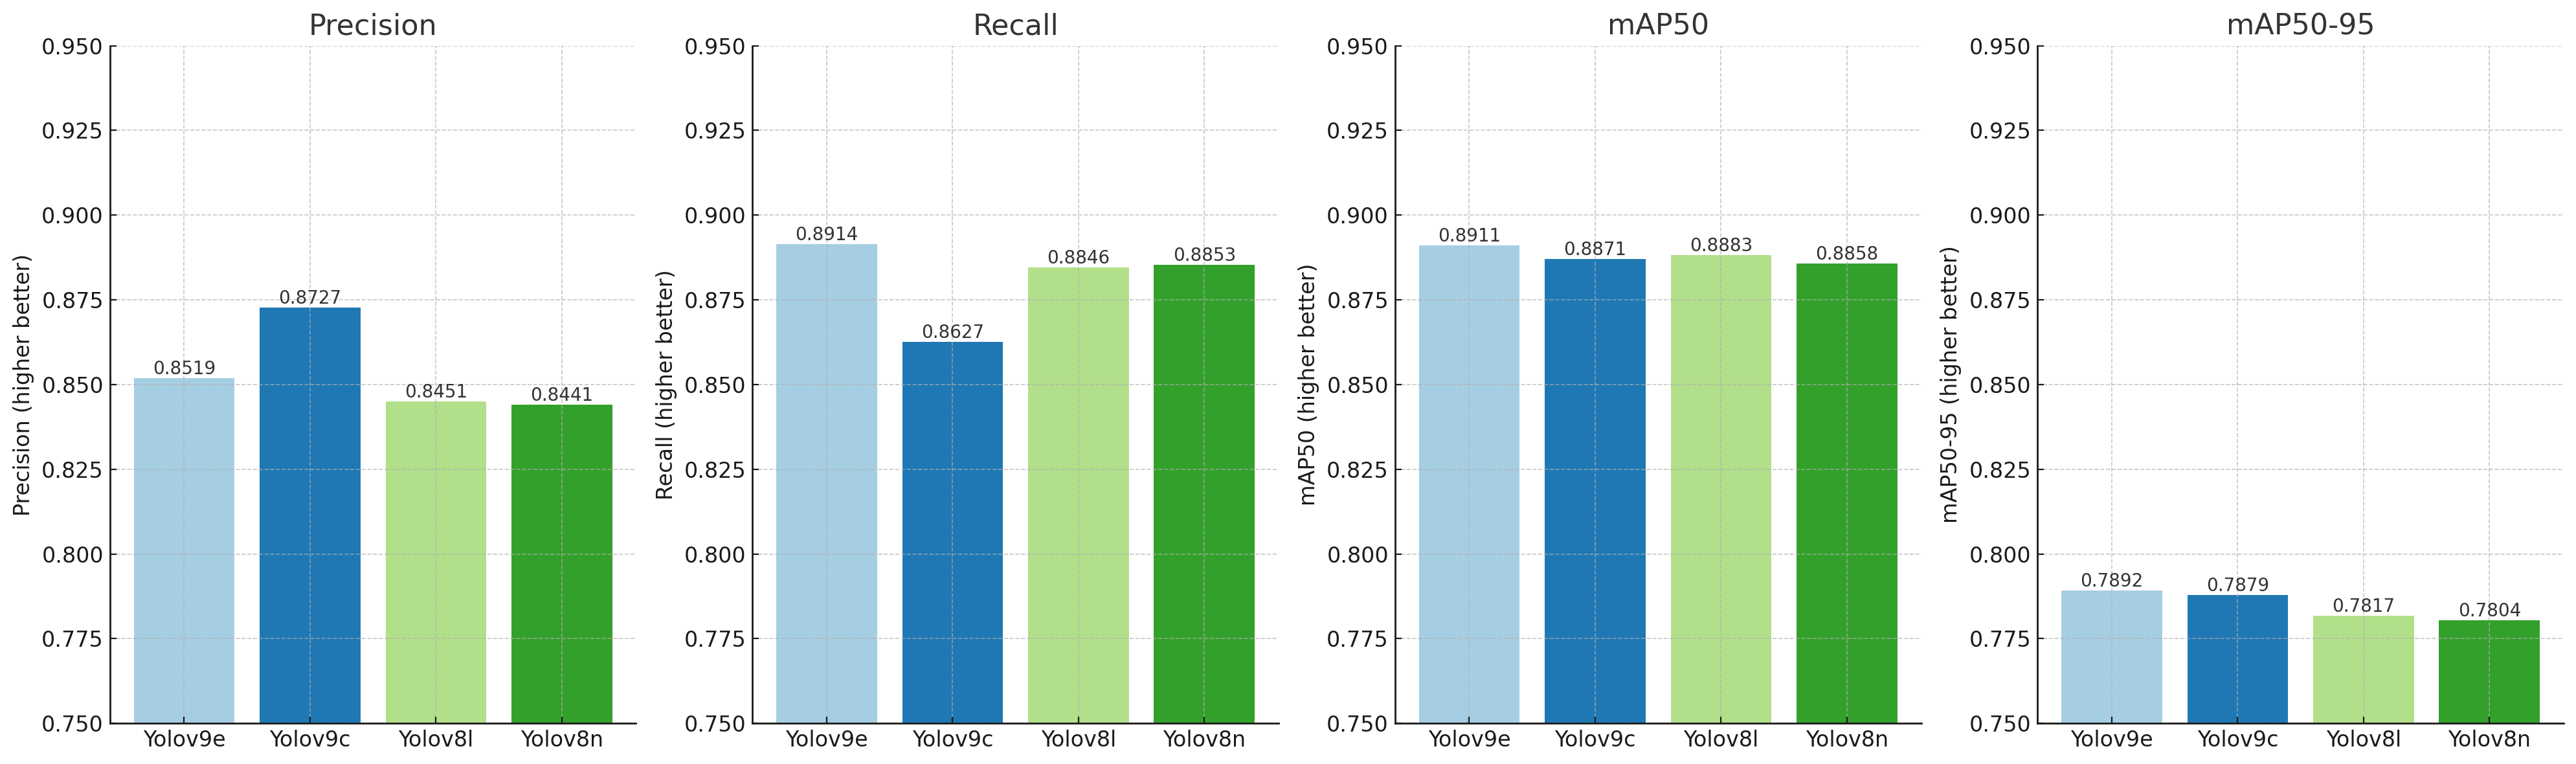
\includegraphics[width=\linewidth]{objectdetectie_yolo_metrics_bigger.png}
\newpage
\item \textbf{Vergelijkingen metrieken van verschillende yolo modellen:}
  \begin{itemize}
    \item \textbf{Precisie:}
    \begin{figure}[H]
      \centering
      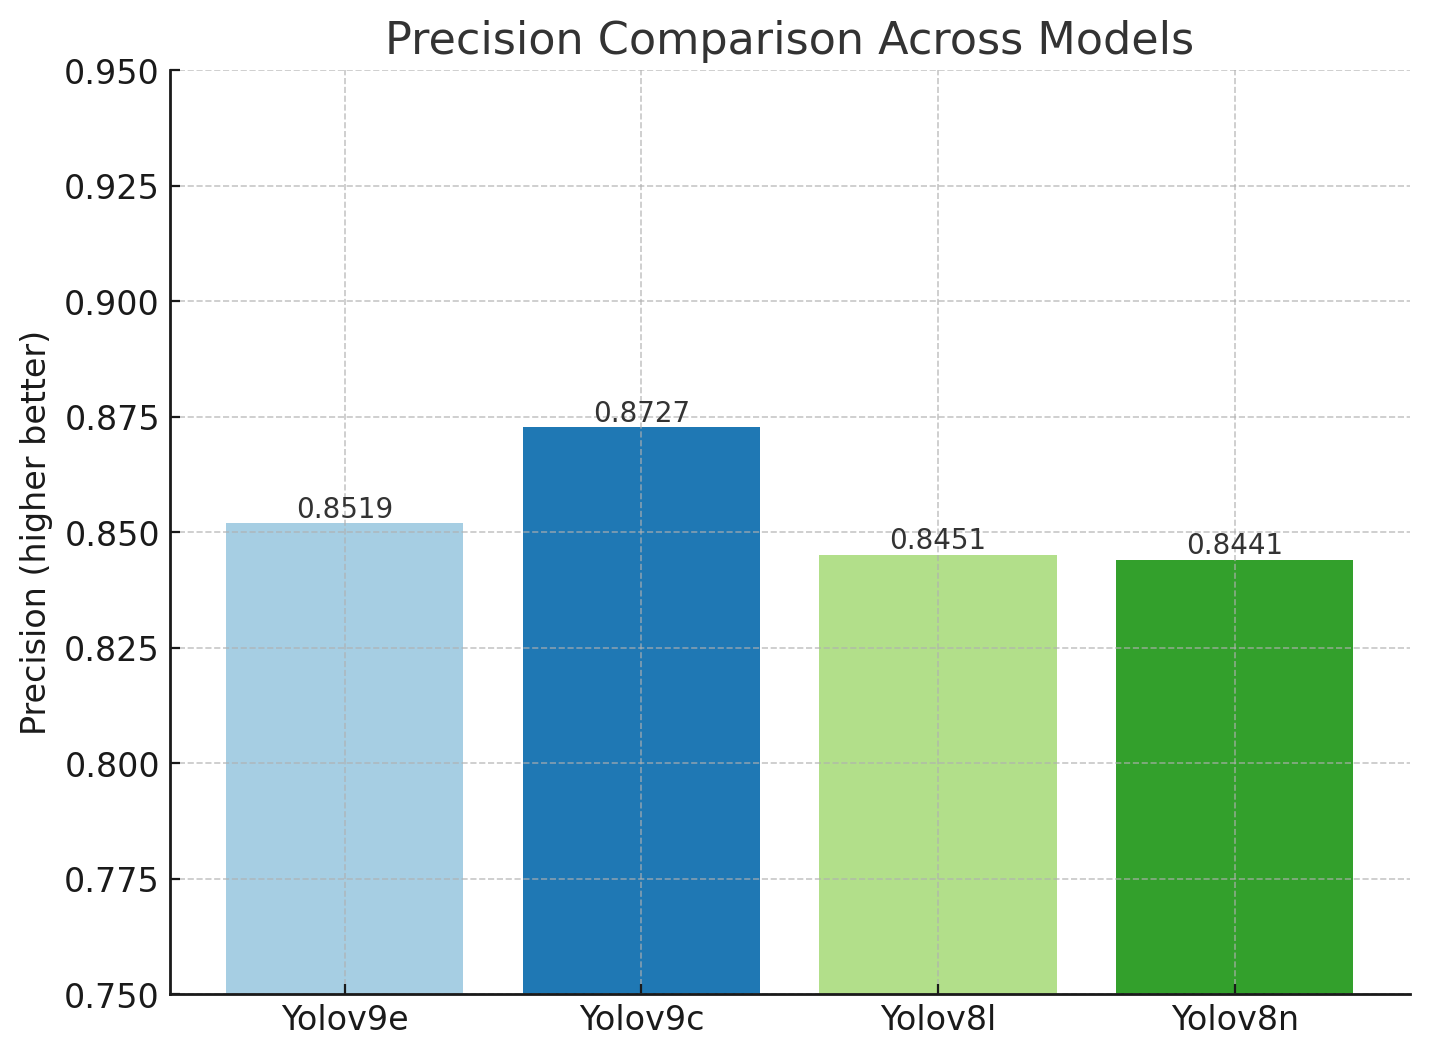
\includegraphics[width=\linewidth]{objectdetectie_yolo_metrics_precision.png}
      \caption{Deze metriek geeft aan welk percentage van de door het model geïdentificeerde objecten correct was. Met andere woorden, het meet de nauwkeurigheid van de positieve voorspellingen van het model. Een hoge precisie betekent dat een groot deel van de door het model gelabelde objecten daadwerkelijk tot de opgegeven klasse behoren.}
      \label{fig:precisie}
    \end{figure}
    \newpage
    \item \textbf{Recall:}
    \begin{figure}[H]
      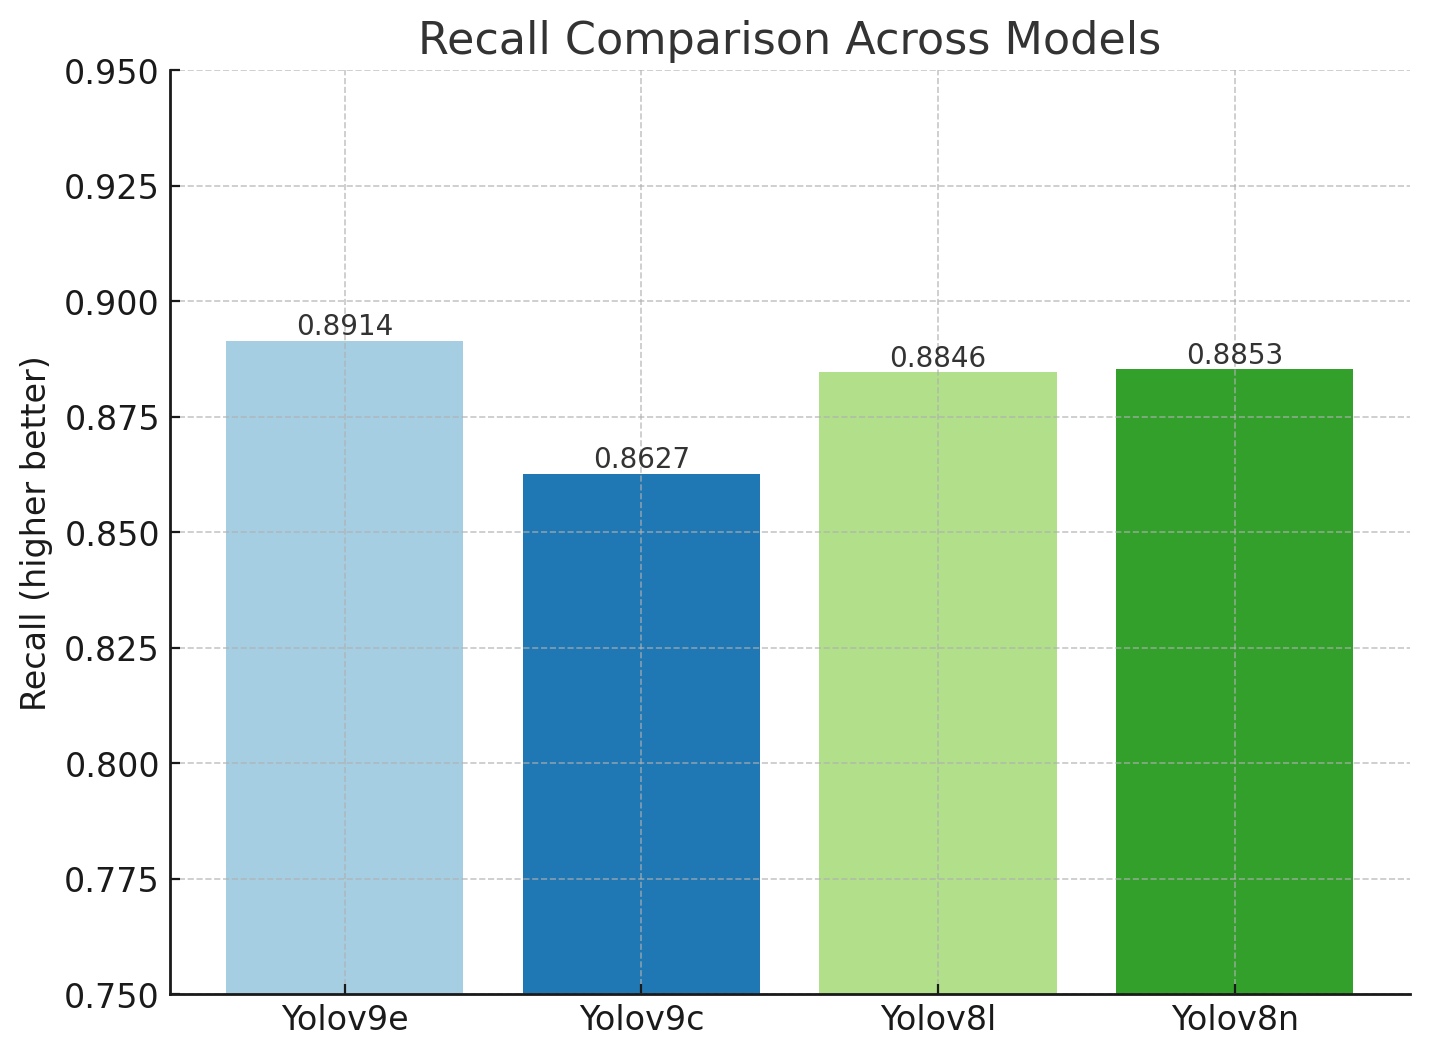
\includegraphics[width=\linewidth]{objectdetectie_yolo_metrics_recall.png}
      \caption{Recall meet hoe goed het model alle relevante gevallen in de dataset kan identificeren. Het is het percentage van de daadwerkelijke positieven dat correct werd geïdentificeerd door het model. Een hoge recall betekent dat het model de meeste van de daadwerkelijke objecten van een bepaalde klasse heeft gedetecteerd.}
      \label{fig:recall}
    \end{figure}
    \newpage
    \item \textbf{mAP50:}
    \begin{figure}[H]
      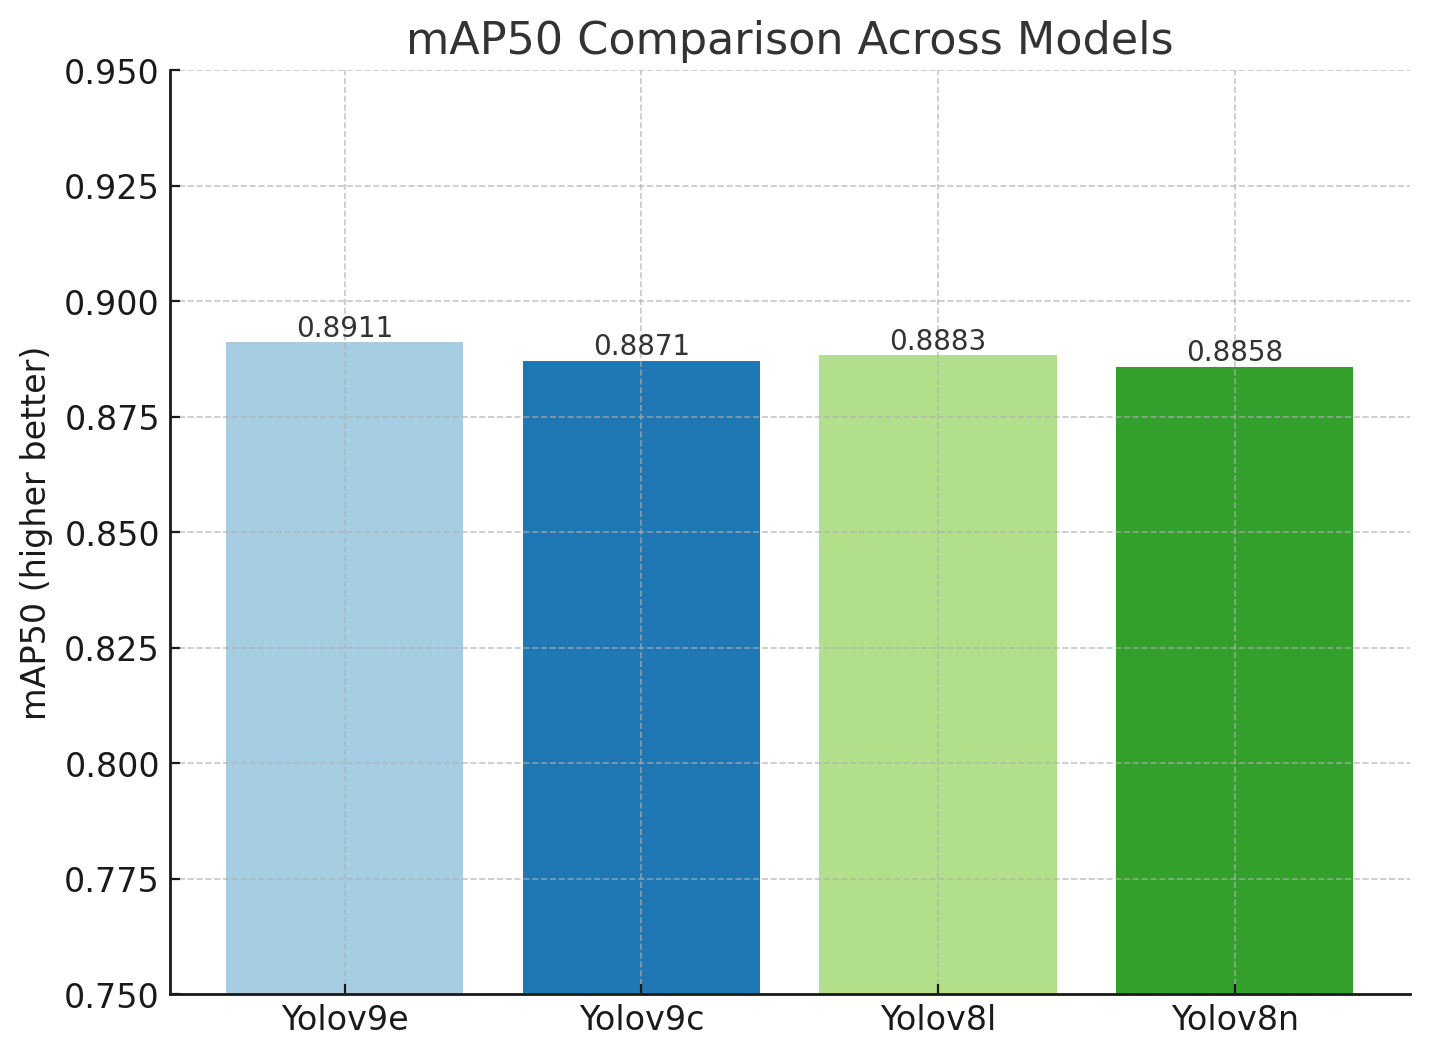
\includegraphics[width=\linewidth]{objectdetectie_yolo_metrics_map50.png}
      \caption{mAP50 (Mean Average Precision at 50\% IOU): Deze metriek wordt gebruikt om de nauwkeurigheid van objectdetectiemodellen te meten. Het is de gemiddelde precisie bij een Intersection Over Union (IOU) drempel van 50\%. IOU is een maatstaf voor de overlap tussen de voorspelde bounding box en de werkelijke bounding box. mAP50 wordt berekend door de gemiddelde precisie over alle klassen en/of query’s te nemen.}
      \label{fig:map50}
    \end{figure}
    \newpage
    \item \textbf{mAP50-95:}
    \begin{figure}[H]
      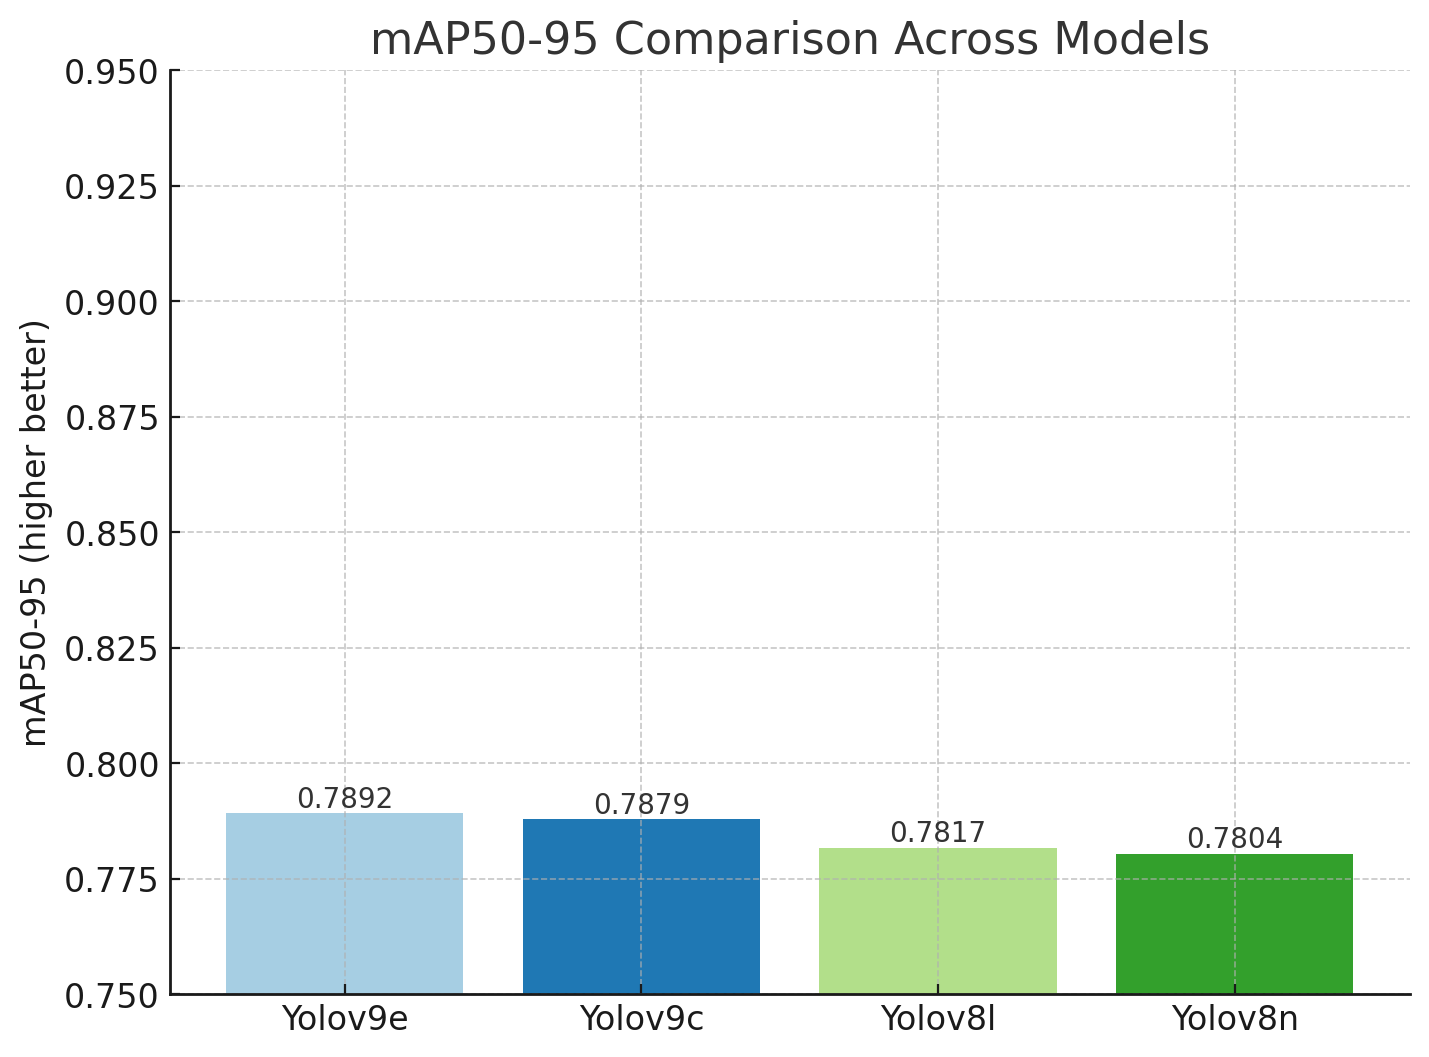
\includegraphics[width=\linewidth]{objectdetectie_yolo_metrics_map5095.png}
      \caption{mAP50-95: Dit is een variant van mAP die de gemiddelde precisie over verschillende IOU-drempels van 50\% tot 95\% (met stappen van 5\%) meet. Deze uitgebreidere metriek is strenger dan mAP50 omdat het consistent goede prestaties over een reeks van overlapdrempels vereist, en geeft een beter beeld van de algehele prestatie van het model.}
      \label{fig:map5095}
    \end{figure}
    \newpage
    \item \textbf{Detectie snelheid (ms):}
    \begin{figure}[H]
      \centering
      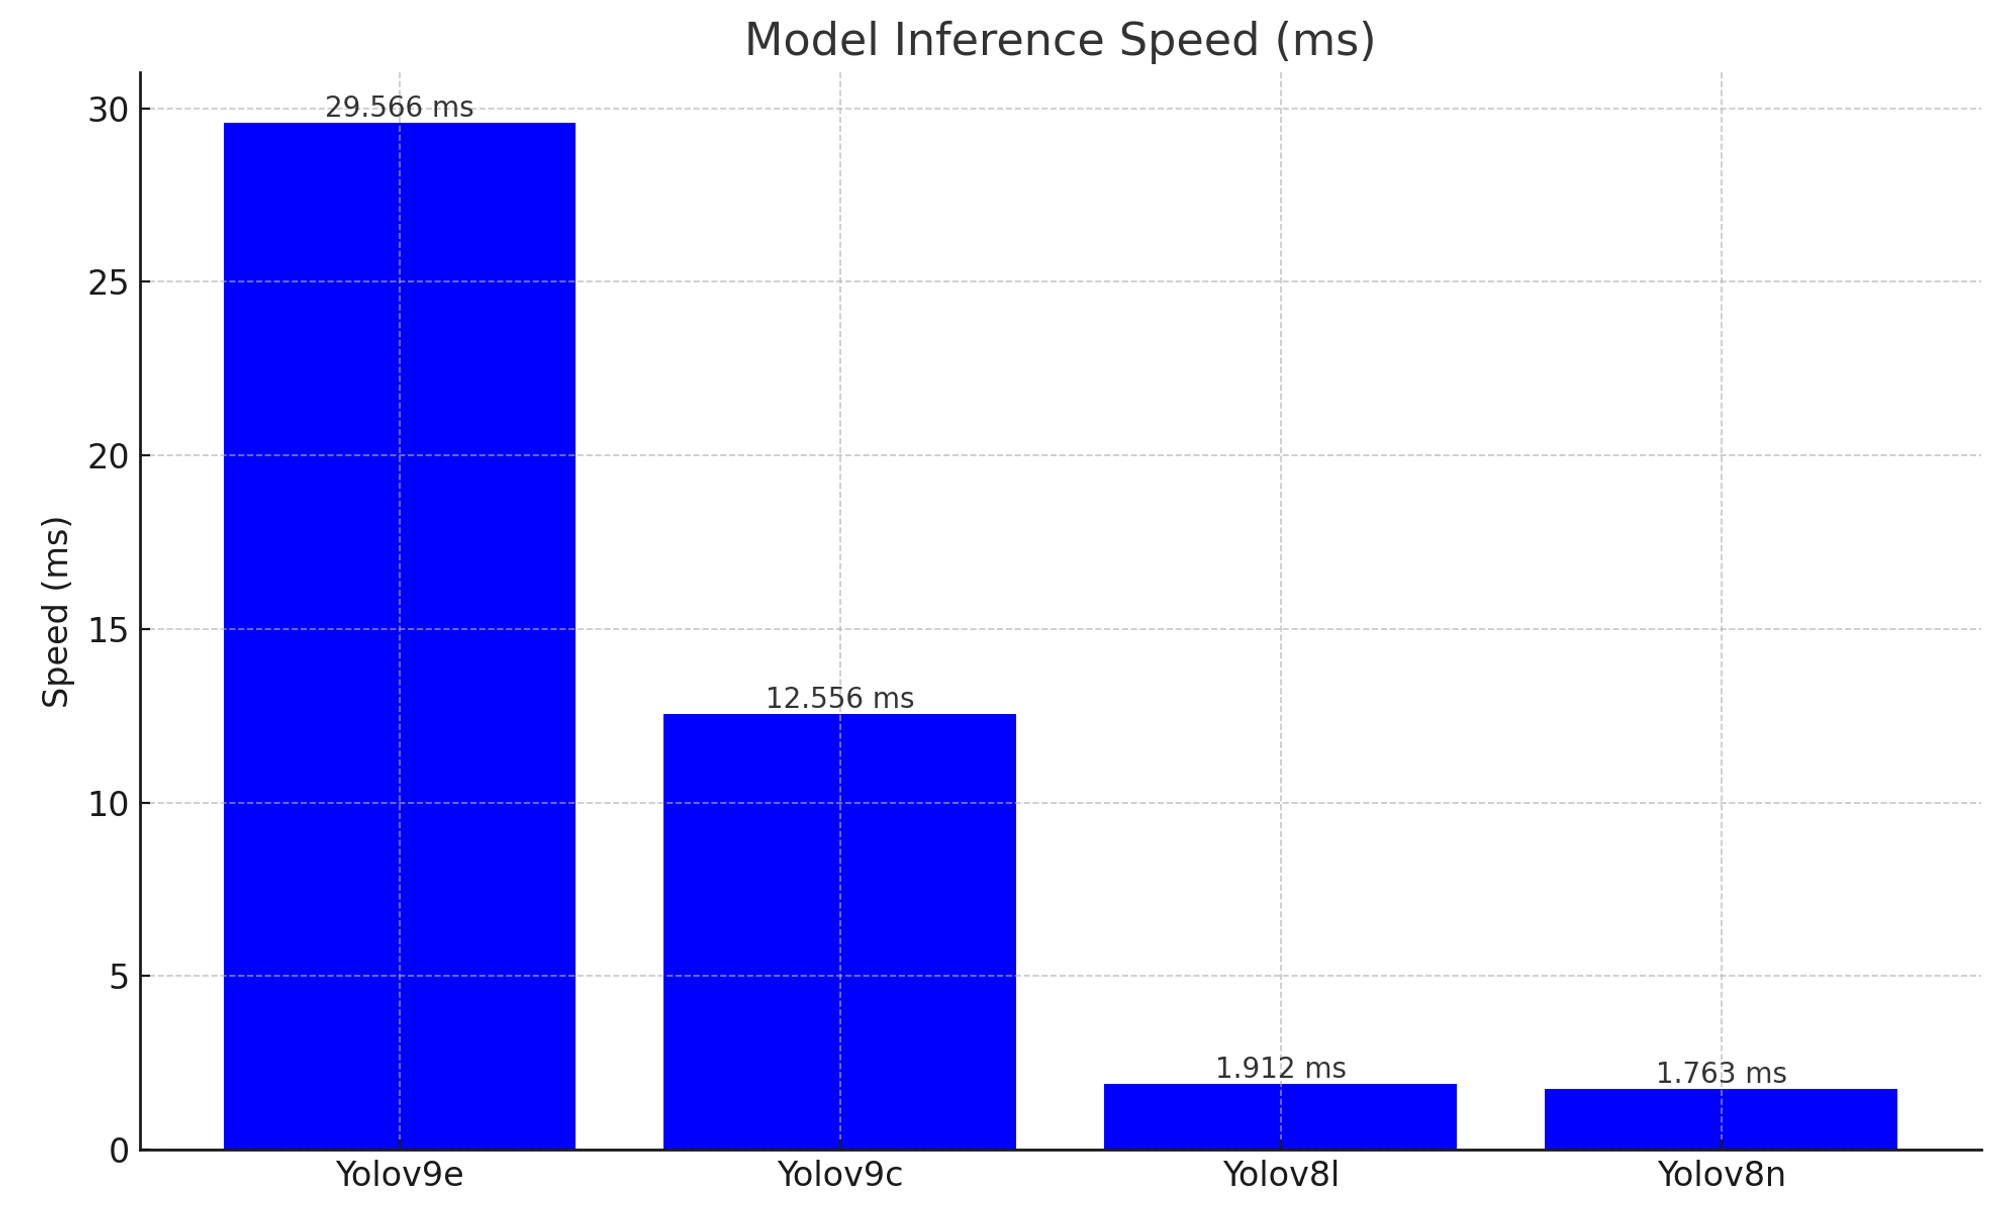
\includegraphics[width=\linewidth]{objectdetectie_yolo_metrics_speed.png}
      \caption{Vergelijking van verwerkingssnelheden tussen verschillende YOLO-modellen. Deze metriek geeft aan hoe snel het model objecten in een afbeelding kan detecteren en classificeren. Een lagere verwerkingstijd betekent dat het model sneller reageert en beter geschikt is voor real-time toepassingen.}
      \label{fig:speed}
    \end{figure}
  \end{itemize}
\end{itemize}
\subsection{Resultaten}
\begin{itemize}
  \item \textbf{Gekozen model:}   Uiteindelijk werd gekozen om verder te gaan met het YOLO-model als de primaire keuze voor objectdetectie in dit onderzoek. Dit besluit was gebaseerd op de superieure prestaties en gebruiksgemak van het model in vergelijking met andere geteste modellen.
  \item \textbf{Gekozen yolo model:} Na een uitgebreide evaluatie van verschillende YOLO-modellen werd besloten om het YOLOv8large-model te gebruiken als de primaire keuze voor objectdetectie in dit onderzoek. Dit besluit was gebaseerd op een evenwicht tussen prestaties en snellere verwerkingstijd, wat essentieel is voor real-time toepassingen.
\end{itemize}
\newline
\begin{figure}[H]
  \centering
  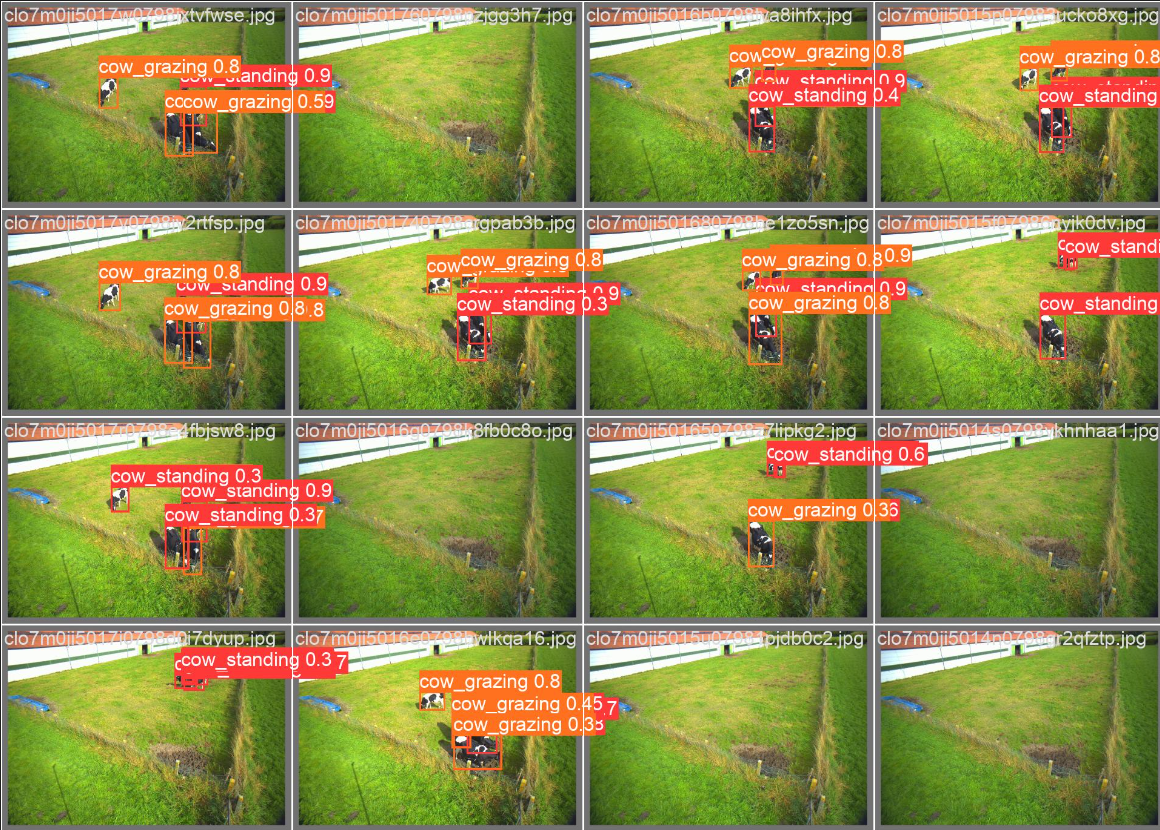
\includegraphics[width=\linewidth]{objectdetectie_yolo.png}
  \caption{Resultaten van yolov8large model na training.}
  \label{fig:yolo}
\end{figure}
\newline